% % Second Chapter : Theoritical Approach
%
% Master Thesis: Calibration and fusion of stereo cameras and optical-range finder sensors
% for in-space localization and mapping
%
% Achieved at Space System Lab, M.I.T.
% Supervisor: Alvar Saenz-Otero, Daniel Alazard
%
% Institut Sup�rieur de l'A�ronautique et de l'Espace
% Major: Telecommunications et r�seaux - Syst�mes Spatiaux et Lanceurs
% Gabriel Urbain - October 2014
%%

\chapter{Theoretical Approach}

In this chapter, we will try to give the reader all the theoretical tools to understand the algorithm development carried out in this project. The first section aims at reminding background models and theories but we will assume the reader to have basics in mechanics of the rigid body, optics, image processing, numerical analysis and computer sciences.
Section two focuses on calibration algorithm. It reviews solutions found in the literature to calibrate separately stereoscopic cameras and TOF camera but also describes the implementation and adaptation of a new algorithm proposed in \cite{stereo_tof_fusion_proba} to calibrate the whole TOF and stereo cameras system while taking advantage of each sensors characteristics.
Finally, the last section analyzes the core implementation of the fusion algorithm tested in this project, try to set out arguments to the choices that have been made and describes each parts in details.

\section{Background}
Before going into further details into the algorithms breakdown, it may be necessary to clarify the models employed throughout this document. Indeed, to simplify the sensor fusion analysis and implementation, we will have to make numerous simplifications and hypothesis about the camera models that we shall remember in Chapter 4 where experimental results are discussed.

\subsection{Mathematical Notations}
Several coordinates systems are used in this work leading themselves to many different transformations between each others. To give the reader a better overview, this paragraph summarizes the mathematical notations employed in this document.

\paragraph{Coordinates Systems:}

\paragraph{Transformations Matrices:}

\subsection{Pinhole Camera Model}
\label{sec:mono_camera}
According to \cite{epipolar_geometry}, a common representation of a camera is composed of a lens represented by a single pinhole $O$ in the \textit{focal plane }$\mathcal{F}$ and a sensor matrix in the \textit{image plane} $\mathcal{I}$ at a distance $f$ from the focal plane. As represented on figure \ref{fig:cam1}, $O$, also called optical center, is the origin of the world 3D coordinates system $OXYZ$ where $Z$ is perpendicular to the focal plane and directed in the opposite direction of the image plane and $X$ and $Y$ are included in the plane. The pixels on the image plane are localized with a 2D coordinates system $O'U'V'$ where the origin is situated on the lower-right corner of the sensor matrix. The $Z$ axis intersects $\mathcal{I}$ in a point $c' = (c_u', c_v')$ called the \textit{principal point}.

% Figure cam1
\begin{figure}[!htt]
	\begin{center}
		\label{fig:cam1}
		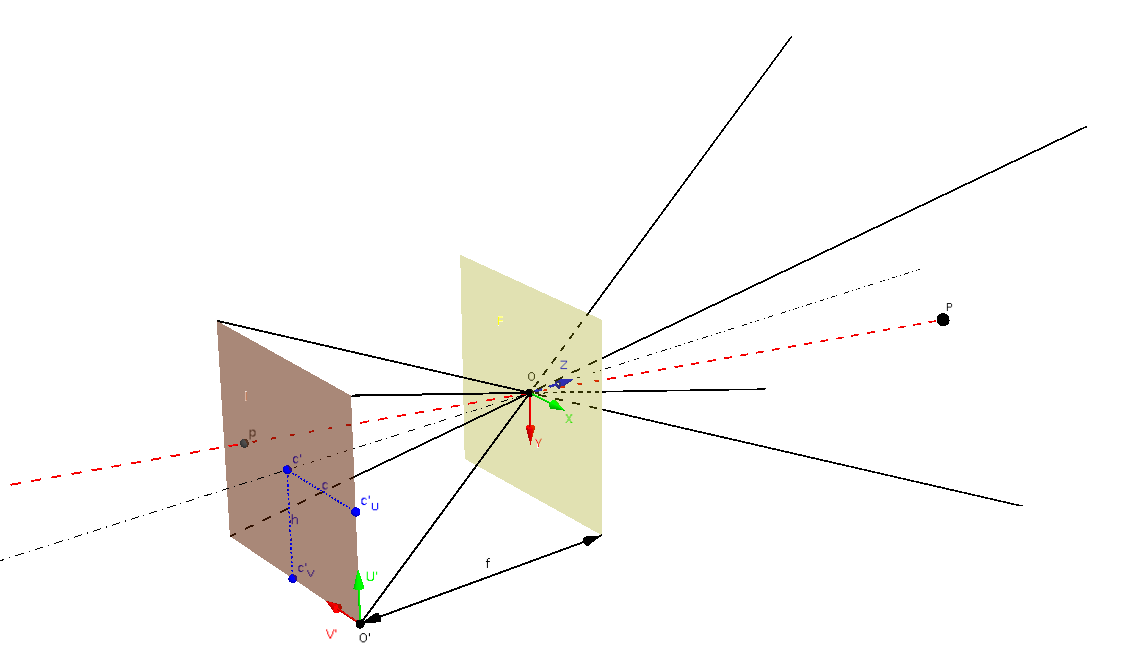
\includegraphics[width=15cm]{img/cam1.png}
		\caption{Geometry of the pinhole model for a single camera}
	\end{center}
\end{figure}

To facilitate the representation, we can consider a \textit{virtual image plane} at a distance $f$ on the positive $Z$ axis, which doesn't change anything to the problem but helps to recreate directly a \textit{projected image} with the same orientation than the real object. We now have a 2D coordinate system $O"UV$ (figure \ref{fig:cam2}).

% Figure cam2
\begin{figure}[!htt]
	\begin{center}
		\label{fig:cam2}
		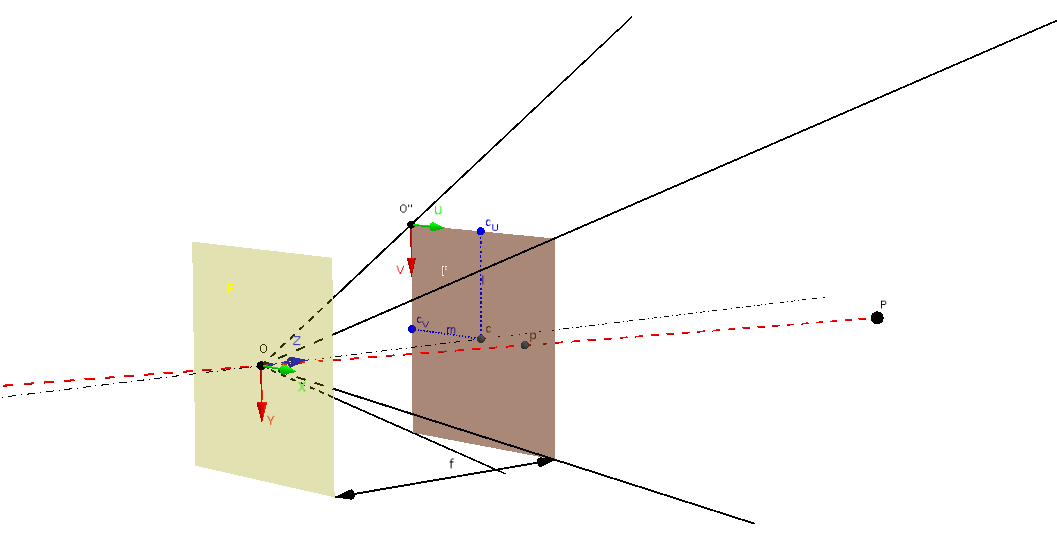
\includegraphics[width=15cm]{img/cam2.png}
		\caption{In this simplified representation, the point P is projected in the virtual plane}
	\end{center}
\end{figure}

In this optimal model, the \textit{intrinsic} geometry of the camera is completely represented by the parameters $f$, $c_x$ and $c_y$ measured in pixels. However, to make the model more realistic, we can introduce extra parameters such as:
\begin{itemize*}
\item The lens enlargement $k$, whose value is different along $u$ and $v$ axis and represented in the model by coordinates $f_u = k_u * f$ and $f_v = k_v * f$
\item The skew $s_{uv}$, assessing the non-orthogonality between rows and columns of the sensor photosensitive cells.
\end{itemize*}
Those five parameters $f_u$, $f_v$, $c_u$, $c_v$, $s_{uv}$ constitute what we call the \textit{intrinsic matrix} of the camera:
\begin{equation}
K =  \begin{pmatrix}
	f_u & s_{uv} & c_u\\
	0 & f_v & c_v\\
	0 & 0 & 1
	\end{pmatrix}
\end{equation}

Therefore, we can write the affine transformation linking a \textit{world point}, represented by its \textit{homogeneous coordinates} in the camera 3D coordinates system and a \textit{projected point} represented by its \textit{homogeneous coordinates} in the image 2D coordinates system:
\begin{equation}
\label{eq:pinhole}
s \begin{pmatrix}[0.8]
u\\
v\\
1
\end{pmatrix}
 = K * \begin{pmatrix}[0.8]
 x\\
 y\\
 z\\
 1
 	\end{pmatrix}
\end{equation}

Finally, the model can be refine to take the distortions into account. As proposed by Brown \cite{camera_distortion}, the distortion may be divided into radial and tangential and can be represented by a second degree polynomial which map the undistorted and distorted images together thanks to 6 parameters. This will be detailed in section \ref{sec:calib}.\\

One should also notice that the parameters discussed here define the camera mathematical model but performances can be determined as well. For instance, the \textit{Field-Of-View} (FOV) of the camera and the pixel size $\epsilon_p$ of the photosensitive cells (sometimes given by the pixel density, measured in pix/meters) are two characteristics to measure camera performances.

\subsection{Stereoscopic Cameras Model}
\label{sec:stereo_camera}
In the literature, the stereo camera is commonly represented as the assembly of two pinhole model whose focal points are separated by a distance called \textit{baseline}. As in figure \ref{fig:cam_stereo}, we thus have now two 3D coordinate systems $L = O_LX_LY_LZ_L$ and $R = O_RX_RY_RZ_R$.

% Figure cam_stereo
\begin{figure}[!htt]
	\begin{center}
		\label{fig:cam_stereo}
		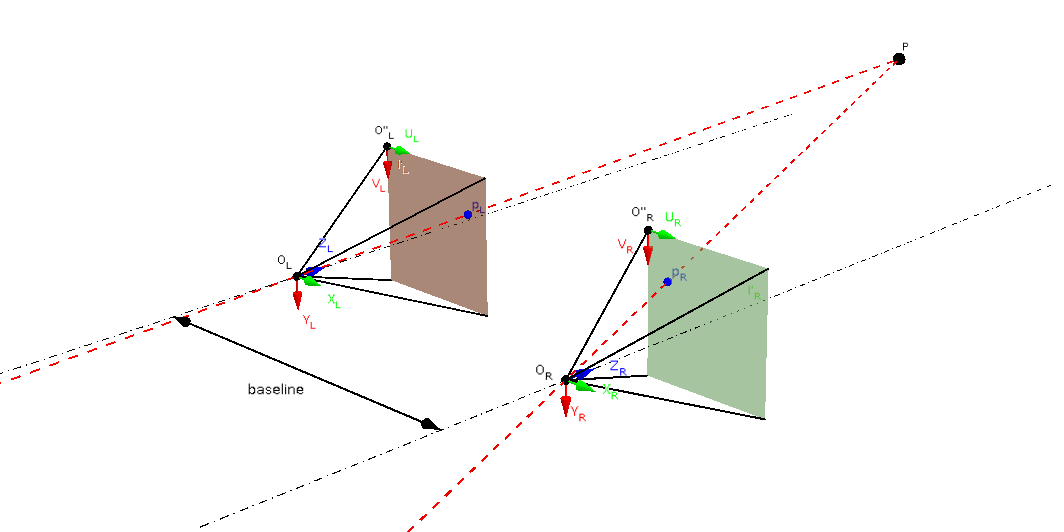
\includegraphics[width=15cm]{img/cam_stereo.png}
		\caption{Model of a stereoscopic cameras assembly}
	\end{center}
\end{figure}

\subsubsection{Projection}
We can still use the model developed in the precedent paragraph the rotation and the translation between $L$ and $R$ must be taken into account when a point is represented in 3D. An \textit{extrincic matrix} is then defined to perform that transformation:
\begin{equation}
M =  \begin{pmatrix}
	r_{X,X'} & r_{X,Y'} & r_{X,Z'} & t_{X}\\
	r_{Y,X'} & r_{Y,Y'} & r_{Y,Z'} & t_{Y}\\
	r_{Z,X'} & r_{Z,Y'} & r_{Z,Z'} & t_{Z}
	\end{pmatrix}
\end{equation}

Which gives:
\begin{equation}
s \begin{pmatrix}
u\\
v\\
1
\end{pmatrix}
 = K * M * \begin{pmatrix}[0.8]
 x\\
 y\\
 z\\
 1
 	\end{pmatrix} = P * \begin{pmatrix}[0.8]
 	 x\\
 	 y\\
 	 z\\
 	 1
 	 	\end{pmatrix}
\end{equation}

Where $P$ is also called the \textit{projection matrix}.

When we write the equations for both left and right cameras, the \textit{extrinsic matrix} can either refer to a third coordinates system, either to $L$ or $R$. In the last case, one of the two $M$ matrix is useless. For instance, if we consider the world coordinates system as $L$, we now write:
\begin{equation}
\label{eq:stereo}
\begin{cases}
s \begin{pmatrix}[0.8]
	u_L\\
	v_L\\
	1
	\end{pmatrix}
= K_L * \begin{pmatrix}[0.8]
	x\\
	y\\
	z\\
	1
	\end{pmatrix}\\
s \begin{pmatrix}[0.8]
	u_R\\
	v_R\\
	1
	\end{pmatrix}
= K_R * M_R * \begin{pmatrix}[0.8]
	x\\
	y\\
	z\\
	1
	\end{pmatrix}
\end{cases}
\end{equation}

As for the camera model, those equations can be used to compute directly the $(u_L, v_L)$ and $(u_R,v_R)$ coordinates from the 3D coordinates of a point with the knowledge of \textit{intrinsic} and \textit{extrinsic} matrices for both cameras. This process is known as \textit{\textbf{projection}}.

\subsubsection{Triangulation}
Intuitively, if inverting the pinhole equation was not directly useful with a mono camera because there was one degree of freedom remaining, we can invert the stereo cameras model to find the 3D coordinates from the projected points in $L$ and $R$. This process, known as \textit{\textbf{triangulation}}, however requires the triangulated points to respect the \textit{epipolar constraint} to give coherent results \cite{multiple_view}, \textbf{i.e.} $(u_L,v_L)$ and $(u_R, v_R)$ must be defined such as the two \textit{epipolar rays} from $L$ and $R$ cross in one point in the real world as represented infigure \ref{fig:cam_stereo}.

Practically, in the 3D reconstruction from stereo sensors problem, the points $p_L = (u_L, v_L)$ and $p_R = (u_R, v_R)$ in the focal images are found using image processing techniques, as developed in \ref{subsec:fusion:overview}. The precision of this method, the accuracy of the physical sensors, the precision of the calibration matrices, the numerical errors,... Everything make this constraint difficult to respect. We can therefore consider two ways to overcome this issue:
\paragraph{Simplify the problem}: In the first option, we suppose the cameras to be perfectly aligned in $Y$ and $Z$ coordinates, the \textit{baseline} is measured on the $X$ axis. Thus, \textit{epipolar lines} are totally included in $XZ$ planes for each points and as soon as those one are visible in left and right images, they will cross for sure. This leads to simplified projection matrices:
\begin{equation}
P_L = \begin{pmatrix}
	f_u & 0 & c_u & 0\\
	0 & f_v & c_v & 0\\
	0 & 0 & 0 & 0
	\end{pmatrix}
\end{equation}
\begin{equation}
P_R = \begin{pmatrix}
	f_u & 0 & c_u & T_R\\
	0 & f_v & c_v & 0\\
	0 & 0 & 0 & 0
	\end{pmatrix}
\end{equation}

\paragraph{Minimize errors}: The other solution is to keep an elaborate model where left and right cameras can be misaligned but try to minimize the sum of euclidean errors when we are triangulating many points. Various algorithm concerning the subject have been analyzed in \cite{multiple_view} or \cite{triangulation}.

The two kinds of \textit{triangulation} and \textit{projection} methods have been implemented in the stereo cameras software but this thesis mostly focus on the first one for it is easier to implement and give sufficient results with VERTIGO \cite{muggler_phd}.

\subsection{Optical Range Finder Model}
A Time-Of-Flight camera (TOF), also called Optical Range Finder (ORF) in this document, is a class of LIDAR that can measure an entire 3D scene in real-time (more than 25 FPS) \cite{TOF_principle}\cite{TOF}. As shown in figure \ref{fig:cam_orf} modulated light bursts illuminating the scene is produced by an IR emitter on the camera, the light is scattered by objects in the scene and a fast CMOS sensor synchronized with the emitter sample the received pulse and retrieve its phase. For each pixel, a distance camera-object can be compute as:
\begin{equation}
d = \dfrac{c}{2}.\dfrac{\Delta\phi}{2 \pi f}
\end{equation}
Where:
\begin{itemize*}
\item $\Delta \phi$ is the phase shift between the emitted and received light
\item $c$ is the light speed: $299 792 458 m/s$
\item $f$ is the IR modulation frequency which has been set to $15MHz$ in our experiments
\end{itemize*}
Which also means that the camera maximal range $D$ is equal to $10m$.

% Figure cam_orf
\begin{figure}[!htt]
	\begin{center}
		\label{fig:cam_orf}
		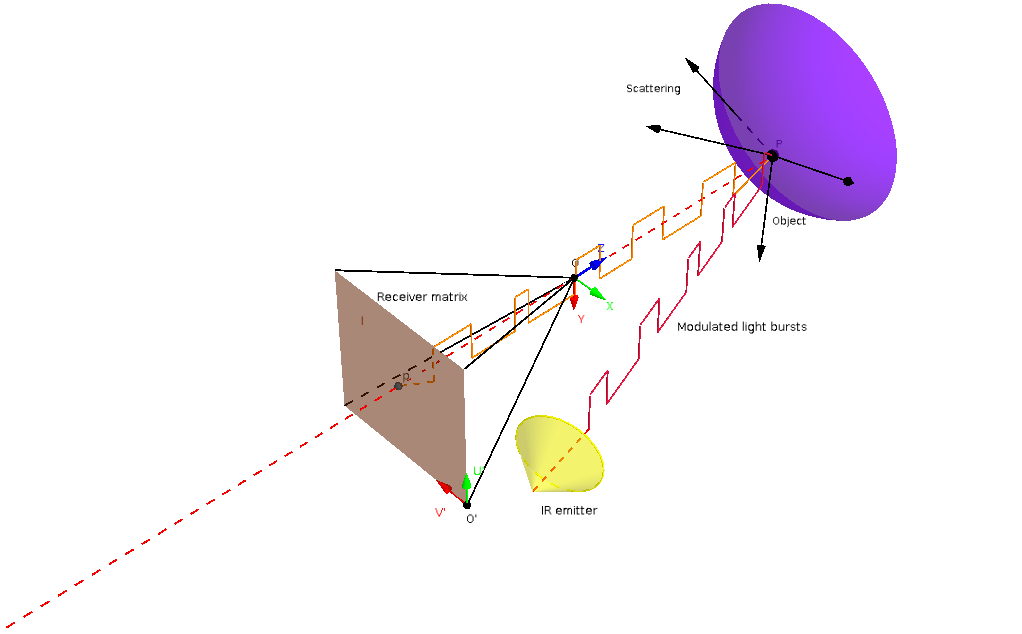
\includegraphics[width=14cm]{img/cam_orf.png}
		\caption{Principle of a time-of-flight camera. The pinhole model is still applicable for the geometry but the measurement of the phase allows to create a new image: the \textit{depth map} $D_T$}
	\end{center}
\end{figure}

In addition to the \textit{depth map} $D_T$, two other images can be extracted from the sensor. In figure \ref{fig:cam_orf_2} provided in the Data Sheet of the camera we are using \cite{SR4k_manual}, $A$ is a measure of the modulated signal amplitude and helps to compute a \textit{confidence map} $C_T$ (the larger $A$, the better confidence on the measure); $B$ is a measure of the mean signal amplitude and gives a \textit{visual image} $V_T$ very similar to the one we can have with traditional black and white cameras.

% Figure cam_orf_2
\begin{figure}[!htt]
	\begin{center}
		\label{fig:cam_orf_2}
		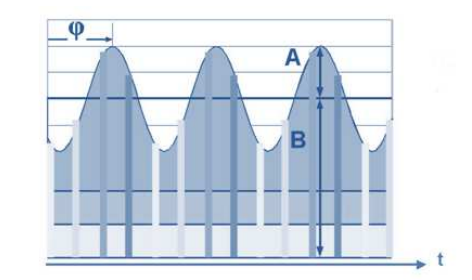
\includegraphics[width=12cm]{img/cam_orf_2.png}
		\caption{The received modulated IR signal is sampled and form the parameters $A$, $B$ and$\Delta \phi$ three images can be computed: \textit{depth map} $D_T$, \textit{confidence map} $C_T$ and \textit{visual image} $V_T$ - \textit{Mesa Imaging SR4k Data Sheet \cite{SR4k_manual}}}
	\end{center}
\end{figure}




\section{Calibration Algorithm}
\label{sec:calib}
\subsection{Literature Overview}
The calibration is a process that aims at finding the most accurate \textit{instrinsic} and \textit{extrinsic} matrices of the pinhole model described in sections \ref{sec:mono_camera} and \ref{sec:stereo_camera} without any prior knowledge of the camera geometry. A precise camera calibration constitutes an important problem since it determines the accuracy of the results. Thus, numerous alternate methods have been developed to guarantee the best possible calibration. According to \cite{intrinsic_calibration}, this process can be divided into three categories:
\begin{itemize*}
\item \textbf{3D object-based calibration}: The known geometry of a 3D object as well as its projection are used to compute the best matrices that verify the pinhole equation \ref{eq:pinhole}. It requires however the presence an accurate 3D calibration target for each calibration.
\item \textbf{Self-calibration}: No object is used but the rigidity of a static environment induces enough constraints to estimate the calibration parameters. If this is very flexible, it is still not always reliable as a lot of initial parameters has to be estimated.
\item \textbf{2D pattern-based calibration}: This third category is a compromise of flexibility as it requires only a 2D pattern like a checkerboard and reliability the solution always converges.
\end{itemize*}
\subsubsection{ORF calibration}
Calibrating the ORF can be seen as a single camera calibration as it involves only the estimation of the \textit{intrinsic matrix}. Different methods has been proposed in \cite{tof_calibration} or \cite{tof_calibration_2}. Due to its success, the Brown method presented in \cite{intrinsic_calib} and \cite{intrinsic_calib_1} will be considered. 
Apart from the \textit{intrinsic} calibration, we shall however notice that \cite{stereo_tof_fusion_proba} and \cite{tof_calibration_1} explain that we shall correct the systematic depth measurement error and this can be realized with a polynomial correction functional approach.
\subsubsection{Stereoscopic cameras calibration}
This category is relatively old, which is an advantage since we can find numerous efficient ways to realize them in literature. For example, in the VERTIGO project, the Brown method \cite{camera_calibration} has been tested through the \textit{OpenCV} libraries \cite{opencv} leading to satisfying results \cite{vertigo_phd}.
\subsubsection{ORF-stereo system calibration}
This last category aims at finding \textit{extrinsic matrices} between the ORF camera and the stereo cameras assembly. Since the problem is quite recent, different algorithms have been proposed these last few years in \cite{stereo_tof_fusion_proba}, \cite{stereo_tof_fusion_accuracy}, \cite{tof_calibration_1}. In this paper, we will focus on the algorithm presented in \cite{stereo_tof_fusion_proba} because besides the ORF \textit{visual image} whose space resolution is very low, the process also takes profit of the \textit{depth map} to increase the accuracy.


\subsection{Optical Range Finder Calibration}
As the ORF can be seen as a simple camera, the goal of the process is to find the matrix $K$ in the pinhole equation:
\begin{equation}
\label{eq:pinhole}
s \begin{pmatrix}[0.8]
u_T\\
v_T\\
1
\end{pmatrix}
 = K * \begin{pmatrix}[0.8]
 x_T\\
 y_T\\
 z_T\\
 1
 	\end{pmatrix}
\end{equation}
Let's take a set of world points $P_T^i$ ($i=1...m$) and their projection $p_T^i$. For each $i$, this equation ca be rewritten:
\begin{equation}
\label{eq:K}
p_T^i = \begin{pmatrix}[0.8]
u\\
v
\end{pmatrix}_T^i =  \mathcal{K}(f_x, f_Y, c_u, c_v, s_{uv}, P_T^i)
\end{equation}
If we consider now the distortion model proposed in \cite{camera_distortion}, we can match initial coordinates $(u_{init},v_{init})$ in the \textit{image plan} with \textit{undistorted} coordinates $(u_{corr}, v_{corr})$ in the same plan through the equation:
\begin{equation}
\label{eq:D}
p_{corr}^i = \begin{pmatrix}[0.8]
u\\
v
\end{pmatrix}_{corr}^i =  \mathcal{D}(u_{init}^i, v_{init}^i, k_1, k_2, k_3, k_4, k_5)
\end{equation}
Where:
\begin{equation}
	\begin{cases}
		u_{corr} = u * (1 + k_1 r + k_2 r^4 + k_3 r^6) + 2 k_4 u v_ + k_5 (r^2 + 2 u^2)\\
		v_{corr} = v * (1 + k_1 r + k_2 r^4 + k_3 r^6) + k_4 (r^2 + 2 v^2) + 2 k_5 u v\\
		r = \sqrt{u + v}\\
		u = \dfrac{u_{init}}{z}\\
		v = \dfrac{v_{init}}{z}\\
	\end{cases}
\end{equation}
From \ref{eq:K} and \ref{eq:D}, we can write then:
\begin{equation}
\label{eq:F}
p_T^i = \begin{pmatrix}[0.8]
u\\
v
\end{pmatrix}_T^i =  \mathcal{F}(f_x, f_Y, c_u, c_v, s_{uv}, k_1, k_2, k_3, k_4, k_5, P_T^i)
\end{equation}
Or more simply:
\begin{equation}
\label{eq:F2}
p_T^i =  \mathcal{F}(\theta_T^i)
\end{equation}
If we define $\theta_T^i = (f_x, f_Y, c_u, c_v, s_{uv}, k_1, k_2, k_3, k_4, k_5, P_T^i)$ as the unknown vector.

Practically, all those points $P_T^i$ correspond to the points on a plane pattern (the corner of a checkerboard). Therefore, to find the vector $\theta_T^i$, we detect the checkerboard corners projections $p_T^i$ in the \textit{visual image} $V_T$, we create an initial guess $\hat{\theta}_T^i$ for each point and we solve the constrained iterative least square problem:
\begin{equation}
\label{eq:calib_min}
\theta_T^i = \mathtt{arg} \mathsf{min}{\sum_{i=1}^m ||\mathcal{F}(\hat{\theta}_T^i) - p_T^i||^2}
\end{equation}
\hspace{30pt}Where constraints are:
\hspace{30pt}\begin{itemize*}
\item \textit{All points are in the same plane}
\item \textit{The distance between two consecutive points is known}
\end{itemize*}
As the iterative algorithm used to solve the problem \ref{eq:calib_min} has been detailed in \cite{intrinsic_calib} and already implemented in OpenCV, we won't give explained in further details but understanding how the problem is defined will be useful in the following sections.


\subsection{Stereoscopic Cameras Calibration}





\subsection{Multi-Sensors Calibration}
\subsubsection{Checkerboard Points Detection}
\subsubsection{Stereoscopic Triangulation}
\subsubsection{Optical Range Finder Pinhole Inversion}
\subsubsection{Pose Estimation}











\section{Fusion Algorithm}
\subsection{Literature Overview}
The goal of the fusion algorithm is to compute a 3D map of the environment, taking advantage of each sensor features in order to improve the global accuracy. Many articles have studied the realization of stereo and ToF cameras fusion algorithm using various alternate methods. In order to understand more clearly, we can divide them into two categories:
\begin{itemize*}
\item In the first category, the stereo algorithm is performed alone without including the ToF informations. As an output of this algorithm, we obtain a 3D map which can be compared to the ToF 3D map to give a refined solution. This analyze is proposed in \cite{stereo_tof_fusion_realtime} where a final 3D map is deduced from the ToF 3D map and the stereo 3D map by \textit{Winner takes it all} or \textit{Simulated annealing} strategies. According to their results, it gives real-time performances with a computation time lower than one second which is a true asset. In \cite{stereo_tof_fusion_patchlet}, 3D maps are fused along many patchlets areas using a \textit{Gauss-Markov Model}.
\item The second category implies incorporating the 3D information of the ToF sensor directly in the stereo algorithm. Those methods seem to give good results but no information about the processing time is given. In \cite{stereo_tof_fusion_proba}, a full probability model is computed and an estimation maximizing the joint probability is then selected. The same kind of approach is used in \cite{stereo_tof_fusion_accuracy}. In \cite{stereo_tof_fusion}, the ToF data are exploited in the initialization phase of a \textit{Dynamic Programming (DP)} algorithm developed in \cite{stereo_algorithm_KUL}. In another field of application, \cite{stereo_tof_fusion_3D_reconstruction} create a joint probability of the two sensors to fulfill a occupancy grid and reconstruct a 3D object from multiple views.
\end{itemize*}
Given those properties, two different methods are considered here. The first one is very simple but may be considered as efficient for real-time applications, the second one gives is assumed to give the best results but need to be tested in real-time applications.


\subsection{Overview}
\label{subsec:fusion:overview}
\subsection{Architecture}
\subsection{Determination of the Points Framed by all Cameras}
\subsection{Optical Range Finder Noise Model}
\subsection{Probabilistic Space Discretization}
\subsection{Optical Range Finder Probabilistic Model}
\subsection{Stereoscopic Cameras Model}
\subsection{Joint Probability Computation}
\subsection{Depth Estimation Selection}
\subsection{3D Coordinates Computation}
\subsection{Point Cloud Creation}